\label{sec:error}
\label{sec:chi2}
%%%%%%%%%%%
In this section various forms of $\chi^2$ 
allowing for the inclusion of systematic and statistical correlations are presented.
They are based on the use of nuisance parameters or on the full covariance matrix.
A schematic picture of $\chi^2$ definitions is displayed in Fig. \ref{fig:chi2}.
\begin{figure}[htb]
% \begin{center}
\centerline{
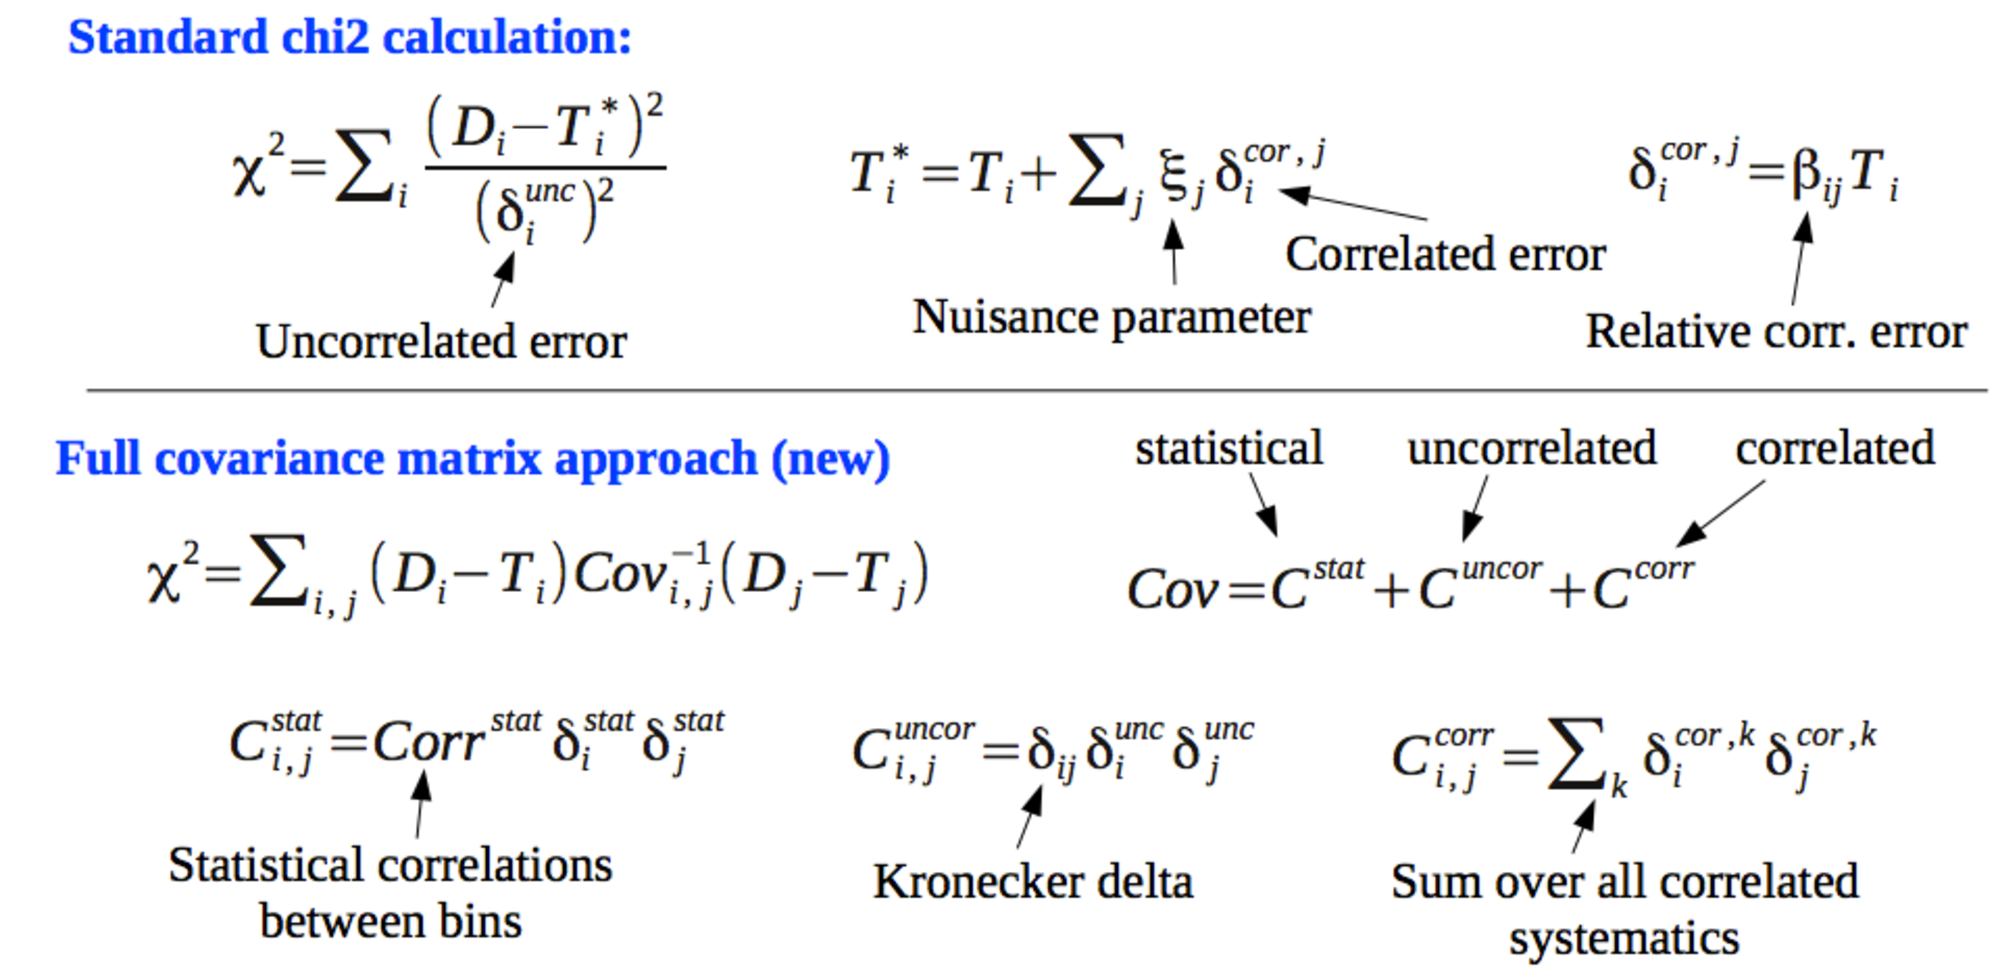
\includegraphics[width=0.75\linewidth]{figures/chi2.pdf}
}
% \end{center}
\caption{Various $\chi^2$ representations in \fitter.}
\label{fig:chi2}
\end{figure}
The description starts with the most simple cases and extends to more evolved forms, which take into account possible biases 
arising from low statistics data.

\subsubsection{Using Nuisance Parameters}
%%%%

\newcommand{\rs}{b}
\newcommand{\ce}{\Gamma}
% \newcommand\ci{l} \newcommand\ck{k}
\newcommand\ci{\alpha} \newcommand\ck{\beta}


In this subsection the focus is on the form of $\chi^2$
using nuisance parameters,
which take into account the correlated systematic error sources.
Several variants are briefly discussed.
For more detailed presentations see Refs. \cite{Stump:2001gu,Botje:2001fx,Aaron:2009bp}.

From the statistical point of view a measurement result, $\mu_i$,
at point $i$ is a random variable which can be modelled as
\begin{equation}
\mu_i = m_i(\boldsymbol{p}) + r_i \sigma_i + \sum_{\ci=1}^{N_\mathrm{syst}} \ce^i_\ci \rs_\ci
\end{equation}
where\\
% $\mu_i$ is the value measured for the $i$-th data point,\\
$m_i(\boldsymbol p)$ is the `true', physical model value depending on parameters $\boldsymbol p = (p_1, p_2,\dots)$,\\
$\sigma_i$ describes the statistical and uncorrelated systematic uncertainties,\\
% $\ce^i_\ci$ are the errors from the $\ci$-th correlated error source,\\
$\ce^i_\ci$ quantifies the sensitivity of the $i$-th measurement to the correlated systematic error source $\ci$,\\
$r_i$ are normal random variables (fluctuating around 0 with unit dispersion).\\
Finally $\rs_\ci$ are nuisance parameters, quantifying the strength of correlated error source $\ci$.

The probability density to obtain a measurement $\boldsymbol \mu = (\mu_1, \mu_2,\dots)$ is proportional to
$e^{-\chi^2(\boldsymbol{m},\boldsymbol{b})/2}$
and the model parameters $\boldsymbol p$ are obtained via the minimisation of $\chi^2$.
To this end the nuisance parameters must be determined.
In the following, different forms of $\chi^2$, as well as different approaches to the nuisance parameters are presented.
% First, a normal distribution of b is assumed, and 
Moreover, the relative rather than absolute uncertainties are used, e.g.
$\ce^i_\ci = \gamma^i_\ci \,\mu_i$ or 
$\sigma_i = \sqrt{\delta_{i,{\rm stat}}^2 +\delta_{i,{\rm uncor}}^2}\,  \mu^i$.
\\

% -o-o-o-o-o-o-o-o-o-o-o-o-o-o-o-o-o-o-o-o-o-o-o-o-o-o-o
\begin{description}
%%%%
\item \bf{Simple Form} \rm

For a single data set, the $\chi^2$ function can be defined in a simple additive form 
\begin{equation}
 \chi^2_{\rm exp}\left(\boldsymbol{m},\boldsymbol{b}\right) = %\\
%~~~=
 \sum_i
 \frac{\left[m^i
- \sum_\ci \gamma^i_\ci \mu^i b_\ci  - {\mu^i} \right]^2}
{ \textstyle \left(\delta_{i,{\rm stat}}\, \mu^i\right)^2 +
\left(\delta_{i,{\rm uncor}}\,  \mu^i\right)^2}
 + \sum_\ci b^2_\ci.
\label{eq:ave}
\end{equation}
%
where the $\boldsymbol{m}$ dependence on $\boldsymbol{p}$ has been suppressed. In the formula,
$\delta_{i,{\rm stat}}$ and $\delta_{i,{\rm uncor}}$
denote the relative statistical  
and relative uncorrelated systematic uncertainties, respectively.
The latin index $i$ runs over the data points, while the greek index $\ci$ runs over the correlated systematic error sources.


% First, a normal distribution of b is assumed, and 
This formula for $\chi^2$, as well as the following ones, is obtained under the assumption of normal distribution of the nuisance parameters. This assumption results in the trailing term,
% $\boldsymbol{b}^2$,
$\sum_\ci b^2_\ci$,
expressing the penalty for correlated shifts away from the central values.


\item \bf{Scaled Form} \rm

Equation~\ref{eq:ave} can be evolved as in~\cite{Aaron:2009bp}:

%
\begin{equation}
 \chi^2_{\rm exp}\left(\boldsymbol{m},\boldsymbol{b}\right) = %\\
%~~~=
 \sum_i
 \frac{\left[m^i
- \sum_\ci \gamma^i_\ci m^i b_\ci  - {\mu^i} \right]^2}
{ \textstyle \delta^2_{i,{\rm stat}}\,\mu^i 
m^i   \prod_\ci \exp \left( -\gamma^i_\ci  b_\ci \right)+
\left(\delta_{i,{\rm uncor}}\,  m^i\right)^2}
 + \sum_\ci b^2_\ci
 \,.
\label{eq:aven}
\end{equation}
%
% Here ${\mu^i}$ is the  measured central value  at a point $i$ 
% with  relative statistical $\delta_{i,{\rm stat}}$ 
% and relative uncorrelated systematic uncertainty $\delta_{i,{\rm uncor}}$.
% Further, 
% $\gamma^i_\ci$ 
% quantifies the sensitivity of the
% measurement ${\mu^i}$
% to the systematic error source $\ci$. 
% The function $\chi^2_{\rm exp}$ depends on the set of
% underlying physical quantities $m^i$ 
% (denoted as the vector $\boldsymbol{m}$) and 
% the set of nuisance parameters $b_\ci$ ($\boldsymbol{b}$) describing the correlated systematic uncertainties.
% The last term, $\boldsymbol{b}^2$, originating from the assumption on the Gaussian distribution of the nuisance parameters,
% expresses the `penalty' for correlated shifts away from the central values.

% This definition of the $\chi^2$ function uses
The above definitions of $\chi^2$ use
%takes into account that
systematic uncertainties that are proportional to the central values 
(multiplicative errors) whereas the statistical errors scale 
with the square roots of the expected number of events. 
Other scaling properties for the statistical and uncorrelated
systematic uncertainties 
are discussed later.

% Note that the physical quantities $\boldsymbol{m}$ are actually
% the functions, $\boldsymbol{m}(\boldsymbol{p})$ of parameters $\boldsymbol{p}$
% introduced by an underlying physical model.


\item \bf{Covariance Matrix} \rm

In the case of correlated (off-diagonal) statistical uncertainties, the $\chi^2$ function
reads
\begin{equation}
\label{eq:chi2gen}
\chi^2_{\rm exp} (\boldsymbol{m},\boldsymbol{b}) = \sum_{ij} \left ( m^i - \sum_\ci \Gamma^i_\ci(m^i)\,b_\ci - \mu^i \right)
  C^{-1}_{{\rm stat}~ij}(m^i,m^j) \left(  m^j - \sum_\ci \Gamma^j_\ci(m^j)\,b_\ci - \mu^j \right) + 
\sum_\ci b^2_\ci \,.
\end{equation}
Here the scaling properties of the correlated systematic uncertainties 
$\Gamma^i_\ci$ and
of the covariance matrix $C_{{\rm stat}}$ are expressed in terms
of $m^i$, and the dependence of $C_{\rm stat}$ on $b_\ci$ is ignored.
The uncorrelated statistical uncertainties if provided are included in the matrix $C_{{\rm stat}}$ in the equation above.

% Using matrix notation we have
% \begin{equation}
% \label{eq:chi2genM}
% \chi^2_{\rm exp} (\boldsymbol{m},\boldsymbol{b}) =
  % \left ( \boldsymbol{m} - \Gamma\,\boldsymbol{b} - \boldsymbol{\mu} \right)^{\rm T}
  % C^{-1}_{{\rm stat}}
  % \left( \boldsymbol{m} - \Gamma\,\boldsymbol{b} - \boldsymbol{\mu} \right) + 
  % \boldsymbol{b}^2 \,.
% \end{equation}
% The last term, $\boldsymbol{b}^2$, in this equation, as well as in Eqs.~\ref{eq:aven},\ref{eq:chi2gen}

Three methods of treatment of the nuisance parameters are implemented in \fitter.
% optimal values
Quadratic dependence of $\chi^2$ on $b_\ci$ allows for a fast determination
of the minimum, without the need to include formal nuisance parameters
% corresponding to the systematic error sources 
into the \textsc{Minuit} minimisation.

In the first method a minimisation of Eq.~\ref{eq:chi2gen} wrt. $b_\ci$ is used to define the covariance
matrix for the systematic uncertainties, which is determined as
\begin{equation}
 C_{{\rm syst}~ij}= \sum_\ci \Gamma^i_\ci \Gamma^j_\ci \,.
\end{equation}
The total covariance matrix is given by the sum of the statistical and
systematic covariance matrices
\begin{equation} 
C_{{\rm tot}} = C_{{\rm stat}} + C_{{\rm syst}}\,,
\end{equation}
and the $\chi^2$ function takes the form
\begin{equation} \label{eq:chi2c}
  \chi^2( \boldsymbol{m}) = \sum_{ij} ( m^i - \mu^i)\, C^{-1}_{{\rm tot}~ij} 
  \,( m^j - \mu^j)\,.
\end{equation}
% It is worth noting that thanks to the `penalty' term $\boldsymbol{b}^2$,
% the same result can be obtained by integrating out the nuisance parameters $\boldsymbol{b}$.



The second method is used to determine optimal shifts of the nuisance
parameters at each iteration.
%Here the statistical nature of $\boldsymbol{b}$ is ignored
% and the optimal shifts are obtained by minimising 
%and $\chi^2$ is given by
%Eq.~\ref{eq:chi2gen} 
%without the penalty term $\boldsymbol{b}^2$.
The minimisation wrt. $\boldsymbol{b}$ leads to a system of  linear equations 
\begin{equation} \label{eq:chi2n}
 \sum_\ck \sum_{ij} C^{-1}_{{\rm stat}~ij} \Gamma^i_\ci \Gamma^j_\ck\, b_\ck + b_\ci = \sum_{ij} C^{-1}_{{\rm stat}~ij} \Gamma^i_\ci (m^j - \mu^j)\,,
\end{equation}
where, $1\le \ci \le N_{\rm syst}$, the total number of correlated systematic uncertainties. The methods given by Eq.~\ref{eq:chi2c} and 
Eq.~\ref{eq:chi2n} are equivalent algebraically
but Eq.~\ref{eq:chi2n} is more efficient numerically
when the number of nuisance parameters is smaller than the number of measurements.
Additional advantage of this method is that it provides information on the nuisance parameter shifts and constraints on them 
which could be important for other applications, e.g. PDF profiling (see Section~\ref{sec:profiling}). 

% Finally
In the third approach the nuisance parameters $\boldsymbol{b}$ are excluded from the $\chi^2$ minimisation.  
In this case, which is referred to as the offset method, the minimum is determined for the values of $\boldsymbol{b}$ set to zero
while uncertainties on the parameters $\boldsymbol{p}$ are determined by shifting each nuisance parameter $b_\ci$
by $\pm 1$ (one standard deviation). The total covariance matrix for parameters $p^i$ is determined as 
\begin{equation}
  C^{\rm offset}_{ {\rm par}~ ij} = \sum_{\ci=1}^{N_\mathrm{syst}} \Delta p^i_\ci \Delta p^j_\ci \,,
\end{equation}
where $ \Delta p^i_\ci = 0.5 ( p^i( b_\ci = +1 ) - p^i(b_\ci = -1))$ and the quality of the fit is estimated by 
fixing $\boldsymbol{p}$ to the values determined at the minimum and minimising with respect to $\boldsymbol{b}$.

Finally, all three approaches can be combined together. For example, some of the systematic uncertainties
can be treated using the matrix method while others can be treated using the Hessian method. In this case, the
covariance matrix  $C_{\rm syst}$ is build using the corresponding sub-set of systematic sources and $C_{\rm stat}$ 
is replaced by $C_{\rm stat}+C_{\rm syst}$ in Eq.~\ref{eq:chi2gen}. Similarly, some of the systematic uncertainties
can be treated using offset method and then $C^{\rm total}_{ {\rm par}} = C^{\rm Hessian}_{\rm par} + C^{\rm offset}_{\rm par}$
where offset and Hessian covariance matrices are calculated using corresponding systematic error sources.

\goodbreak
\item \textbf{Bias corrections}

The correlated and uncorrelated systematic uncertainties can be treated as additive,  $\Gamma^i_\ci(m^i) = \gamma^i_\ci \mu^i$
or multiplicative, $\Gamma^i_\ci(m^i) = \gamma^i_\ci m^i$. 
% A LogNormal treatment in which 
% $ \mu^i + \sum_\ci \Gamma^i_\ci b_l$ is replaced by $ \mu^i \prod_l \exp( \gamma^i_\ci b_l) $ is foreseen for the
% next release of the \fitter. 

The statistical uncertainties can be treated as additive, $\Delta^i(m^i) = \delta^i \mu^i$  or as Poisson,
$\Delta^i(m^i) = \delta^i \sqrt{\mu^i m^i}$. More complex scaling from Eq.~\ref{eq:aven}, 
which depends on shifts of $b_\ci$, is implemented using an iterative approach: for the first iteration $b_\ci =0$ 
 is used to determine values of $b_\ci$ which are then applied in the second iteration. The statistical covariance
matrix is scaled in a similar manner. In this case the correlation matrix is assumed to be fixed, the diagonal
elements are updated using the prescription describe above and the covariance matrix is rescaled accordingly.

The modifications of the covariance matrix at each iteration of the \textsc{Minuit} minimisation may lead to systematic
biases. There are two approaches that can be used to avoid these biases. In the first approach the covariance matrix is calculated
using the expected values at the first iteration of the minimisation and kept fixed to these values for further
iterations. This method requires several repetitions of the minimisation, to ensure that values close to optimal
are obtained already at the first iteration. The second method~\cite{h1:2012kk} modifies the $\chi^2$ function by adding a term
corresponding to a non constant value of the covariance matrix:
\begin{equation}
 \chi^2_{\rm log} = 2 \log \frac{\Delta^i(m^i)}{\Delta^i(\mu^i)} 
\end{equation}  
\end{description}
% -o-o-o-o-o-o-o-o-o-o-o-o-o-o-o-o-o-o-o-o-o-o-o-o-o-o-o


\subsubsection{\fitter implementation}

\begin{table}
\begin{center}
\begin{tabular}{ccccc} 
\hline
{\sc CHI2SettingsName:}   & {\sc StatScale} & {\sc UncorSysScale} & {\sc CorSysScale} & Scaling rule \\
\hline
{\sc CHI2Settings}       &                 &                     &                   &              \\
\hline
  {\sc Poisson}   &  $+$  &  $+$  &  $-$  & $\sqrt{ m^i \mu^i}$ \\
  {\sc Linear}    & $-$   &  $+$  &  $+$  & $m^i$               \\
  {\sc NoRescale} & $+$   &  $+$  &  $+$  & $\mu^i$   \\
  {\sc LogNorm}   &  \multicolumn{4}{c}{Reserved, not implemented} \\
\hline
\end{tabular}
\end{center}
\caption{\label{tab:ErrScale}Global scaling rules for statistical, 
uncorrelated and correlated systematic uncertainties. The scaling
rule is given with respect to corresponding relative uncertainty.
E.g. for the {\sc Poisson} statistical uncertainty the absolute statistical
uncertainty is $\Delta_i = \delta_{i, {\rm stat}}\sqrt{m^i\mu^i}$   }
\end{table}

The form of the $\chi^2$ function and the scaling properties of the 
uncertainties are controlled globally by the {\sc CHI2SettingsName} and
{\sc  Chi2Settings} variables and individually using {\sc ``:''} modifiers.
The global scaling properties of the uncertainties are described in 
Table~\ref{tab:ErrScale}. The global form of the $\chi^2$ function
is defined by the {\sc CorChi2Type} parameter, see   
Table~\ref{tab:Chi2Type}.

The default behavior can be changed for each correlated systematic source by ``:'' modifiers.
They are described in Table~\ref{tab:SystModifier}. The modifiers should appear at the end 
of the systematic source name, e.g. {\sc 'H3:M'}. Several modifiers can be used, e.g. {\sc 'H3:M:C'}.

\begin{table}
\begin{center}
\begin{tabular}{cl}
\hline
    {\sc CorChi2Type} value &  Description \\
\hline
  {\sc Hessian}             & Use nuisance parameters.\\
  {\sc Matrix }             & Use covariance matrix. \\
  {\sc Offset }             & Use offset method\\
\hline
\end{tabular}
\end{center}
\caption{\label{tab:Chi2Type}Possible values of the {\sc CorChi2Type} parameter which defines treatment of the correlated systematic uncertainties.}
\end{table}
 
\begin{table}
\begin{center}
\begin{tabular}{cl}
\hline
  Modifier &  Description \\
\hline
   \multicolumn{2}{c}{Scaling properties}\\
  {\sc :M}  &  Multiplicative scaling, $ m^i$ \\
  {\sc :A}  &  Additive scaling, $ \mu^i$ \\
  {\sc :P}  &  Poisson scaling, $ \sqrt{m^i\mu^i}$ \\
   \multicolumn{2}{c}{$\chi^2$ treatment}\\
  {\sc :N}  &  Nuisance parameter treatment \\
  {\sc :C}  &  Covariance matrix treatment \\
  {\sc :O}  &  Offset method treatment \\
  {\sc :E}  &  Nuisance parameter, included in {\sc Minuit} (``External'')\\
\hline
\end{tabular}
\end{center}
\caption{\label{tab:SystModifier}Modifiers for correlated systematic
uncertainty sources.}
\end{table}

The names of systematic error sources are read first from the {\sc ListOfSources} variable of the 
{\sc \&Systematics} namelist, located in the {\sc steering.txt} file. Next the names are read from the
data files following the sequence given by the {\sc InputFileNames} list. The properties of each systematic
error source are defined by its first occurrence. That means that if, for example, {\sc 'H3:M:C'} is defined
in the {\sc ListOfSources} variable, the source {\sc 'H3'} is treated as multiplicative and using covariance
matrix approach regardless definitions in the data files. If, however, {\sc ListOfSources} defines a source
without any modifiers, e.g. {\sc 'H3'}, the default treatment, following the {\sc Chi2Settings} variable is
enforced for this source.
Thus the {\sc ListOfSources } variable is a convenient way to modify behavior of the correlated systematic
sources.

The shifts of the systematic sources are reported in the {\sc Results.txt} file. The uncertainty on the shift
is however estimated only approximately, neglecting the correlation with the theory parameters. An accurate determination
of the uncertainty can be achieved by using the toy MC method (see section~\ref{sec:ToyMC}) or by using {\sc ':E'} 
modifier. In the latter case the systematic source is treated using the {\sc Minuit} minimisation. Note, however,
that this approach can slow the minimisation convergence considerably.

% \begin{description}
% \item \bf{Implementation via \fitter\ } \rm

When {\sc CorChi2Type} is set to {\sc Offset}
all fits are run in a single job, each fit driven by initial parameters read from \verb'minuit.in.txt'.
Two optional parameters can be set in the {\sc CSOffset} namelist, e.g.
% \vspace*{-2.5ex}
\begin{verbatim}
&CSOffset
 CorSysIndex  =  0
 UsePrevFit = 1
&End
\end{verbatim}
\vspace*{-1ex}
% Defaults are set in \verb'read_steer.f'
% and the \verb'CSOffset NAMELIST' is read only when the Offset method is active.
Setting \verb'CorSysIndex' to any value $\in [-N_\mathrm{syst}, N_\mathrm{syst}]$ 
restricts the job to a single fit to data shifted (down or up) by the corresponding correlated error source.
\verb'CorSysIndex' = 0 corresponds to the central fit.
If \verb'CorSysIndex' is omitted then all fits are performed.
% The best way to perform all fits in a single run is 
% to not specify \verb'CorSysIndex' at all 
% (Default: \verb'CorSysIndex = NSYSMAX+1' )
% \vspace{0.4cm}

The parameter {\tt UsePrevFit} determines how to use the results of previous fits,
if such results are present in the \verb'output' folder.
\begin{enumerate}
\item [0 ---]
Do not use any previous fit results (Default)
\item [1 ---]
Use previously obtained parameters as starting values for the current fit.
% For a non-offset fit read initial parameters from \verb'minuit.save.txt';
% for an offset fit 
Read initial parameters from \verb'minuit.save_<CSI>.txt'
 --- e.g.  \verb'minuit.save_001m.txt' for \verb'CorSysIndex' $= -1$.
If the file does not exist and \verb'CorSysIndex' $\neq 0$ try to read
\verb'minuit.save_0.txt'.
\item [2 ---]
Do not perform the fit if a corresponding \verb'Results_<CSI>.txt' file exists,
otherwise switch to mode 1.
\end{enumerate}
% \end{description}

% available as described in appendix~\ref{sec:xFitter}.

%%%%
%\subsubsection{Generalised Scaled Form}

%%%%%%%%%%%
%\subsection{Using Covariance Matrix}
%%%%%%%%%%%%%%%%%%%%%%%%%%%%%

%%%%%%%%%%%
\subsubsection{Monte Carlo Method}
\label{sec:ToyMC}

The PDF uncertainties can be estimated using a Monte Carlo technique \cite{Giele:1998gw, mcmethod2}.
The method consists in preparing replicas of data sets by allowing the central values of the cross sections to 
fluctuate within their systematic and statistical uncertainties taking into account all point-to-point correlations.
The preparation of the data is repeated for a large $N$ ($>100$ times) and for each of these replicas a NLO QCD fit is performed to 
extract the PDF set. The PDF central values and uncertainties are estimated using the mean values and RMS 
over the replicas. 
\subsubsection{Implementation in \fitter\ }
The steering flags to activate the MC method are located in the \tt steering.txt \rm via:

\begin{verbatim}
&MCErrors

  lRAND   = False  
  lRANDDATA = True
  ISeedMC = 123456 
  ! --- Choose what distribution for the random number generator 
  ! STATYPE (SYS_TYPE)  =   1  gauss
  ! STATYPE (SYS_TYPE)  =   2  uniform
  ! STATYPE (SYS_TYPE)  =   3  lognormal
  ! STATYPE (SYS_TYPE)  =   4  poisson (only for lRANDDATA = False !)
  STATYPE =  1
  SYSTYPE =  1
&End
\end{verbatim}
To activate the MC method for error estimation set \tt lRand = True \rm.
To use data (true, default) or theory (false) for the central values of the MC replica
the the flag \tt lRANDDATA \rm is used. The seed for random number generation is selected 
via \tt ISeedMC \rm . The smearing of the uncertainties can be treated differently for correlated 
or uncorrelated source and four distributions are supported for random number generators: Gauss, uniform, lognormal, and Poisson. If the flags are set to $0$ then no smearing is produced.




%%%%%%%%%%%
\subsubsection{Regularisation methods}

Regularisation methods are aiming to study the parametrisation assumptions of PDFs. 
When more flexible parametrisation styles is used the shape of the PDFs must be constrained and various methods are used.
The \fitter\ framework provides the means to study and compare various methods.

%The methods described in this section work for large data sets. 

\begin{description}

\item \bf{Data Driven Regularisation}\rm

This method was first applied by the NNPDF group.
It uses a redundant paremeters and introduces a stopping criterion based on data. This method splits data randomly
into ``fit'' and ``control''  samples. The ``fit'' sample is used to determine the PDF parameters. 
The $\chi^2$ of this sample is observed to decrease semi-monotonically. 
The ``control'' sample is used to protect against over-fitting and for this sample the $\chi^2$ will first decrease 
and then will start to increase due to fluctuation of the data.


\item \bf{External Regularisation based on a penalty term in $\chi^2$} \rm

Another method to constrain the PDF shape is to simply apply a penalty term
to the $\chi^2$ function. 
One method is the so called ``length penalty'' which selects PDF solutions with a smoother shape in $W\approx Q\sqrt{\frac{1-x}{x}}$:
\begin{equation}
L=\int_{W_{min}}^{W_{max}} \sqrt{1+\left(\frac{dxf(W)}{dW}\right)^2}dW
\end{equation}
This method can be applied when using Chebyshev polynomials to parametrise PDFs.
For more details, the reader is invited to consult  reference \cite{Chebyshev}.
This method is implemented in \fitter\ via steering flags under Namelist \tt \&Cheb \rm as follows:
\begin{verbatim}
&Cheb
  ! Set following > 0 to turn on:
   NCHEBGLU = 0   ! number of parameters for the gluon (max 15)
   NCHEBSEA = 0   ! number of parameters for the sea   (max 15)

  ! Cheb. polynomial type: multiply by (1-x) (1) or not (0)  
   ichebtypeGlu = 1 
   ichebtypeSea = 1 

  ! Starting point in x:
   chebxmin = 1.E-5

   ILENPDF  = 0   ! use pdf length constraint

  ! PDF length constraint strength for different PDFs:
   PDFLenWeight = 1., 1., 1., 1., 1.     

  ! Range in W where length constraint is applied:
   WMNLen =  20.
   WMXLen = 320.
&end
\end{verbatim}

Alternatively, when using the flexible parametrisation style a $\chi^2$
penalty term can be applied to account for th deviation from a simpler parametric form, for example
\begin{equation}
\chi^2_{reg}= T\sum_f\left(\left(\frac{D_f}{\Delta_D}\right)^2+ \left(\frac{E_f}{\Delta_E}\right)^2\right),
\end{equation}

with $\Delta D=\Delta E = 100$, such that for large $D$ and $E$ the ratio will approach $1$. 
$T$ is the regularisation parameters, such that for $T=0$ there is no penalty term. 
For large $T$ there is strong penalty.
This method of regularisation is accessed via Namelist: \tt \&ExtraMinimisationParameters \rm
with the name \tt 'Temperature' \rm which is $T$ in the above description.

\end{description}
